\icode[purple]{E-EME-MU-L4-260625-002}
（多选）
 如图三个点电荷分别固定在边长为\(a\)的等边三角形的三个顶点上，电荷量分别为\( + q\)、\( + 2q\)、\( + 2q\)，\(O\)为三角形的中心，此时系统的电势能为\(E_0\)，已知两个带电荷量分别为\(q_1\)、\(q_2\)的点电荷组成和系统的电势能为\(\frac{kq_1q_2}{r^2}\)，\(k\)为静电常量，\(r\)为点电荷之间的距离。以下说法正确的是\paren[]

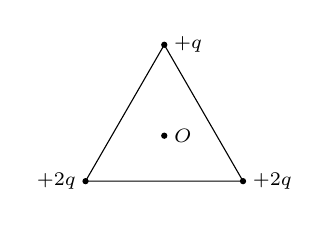
\begin{tikzpicture}[font=\scriptsize]
    \draw (0,0)coordinate(c)node[left]{\( + 2q\)}--++(60:2)coordinate(a)node[right]{\( + q\)}--++(-60:2)coordinate(b)node[right]{\( + 2q\)}--cycle;
    \foreach \c in{a,b,c}
        \fill (\c) circle(.04);
    \fill (30:{2*sqrt(3)/3}) circle(.04)node[right]{\(O\)};
\end{tikzpicture}
\begin{choices}
    \item \(O\)点的场强大小为\(\frac{3kq^2}{a^2}\)
    \item \(O\)点的场强大小为\(\frac{2kq^2}{2a^2}\)
    \item 若取走一个\( + 2q\)的点电荷，系统的电势能将减小\(\frac{E_0}{2}\)
    \item 若取走一个\( + 2q\)的点电荷，系统的电势能将减小\(\frac{E_0}{4}\)
\end{choices}
\begin{answer}
    AD\quad 提示：
\end{answer}